\section{Проектирование системы, разработка языка и алгоритма}

\subsection{Архитектура системы}

Рассмотрим архитектуру системы по модели С4~\cite{c4-model}.

\subsubsection{Взаимодействие систем}

\begin{figure}
  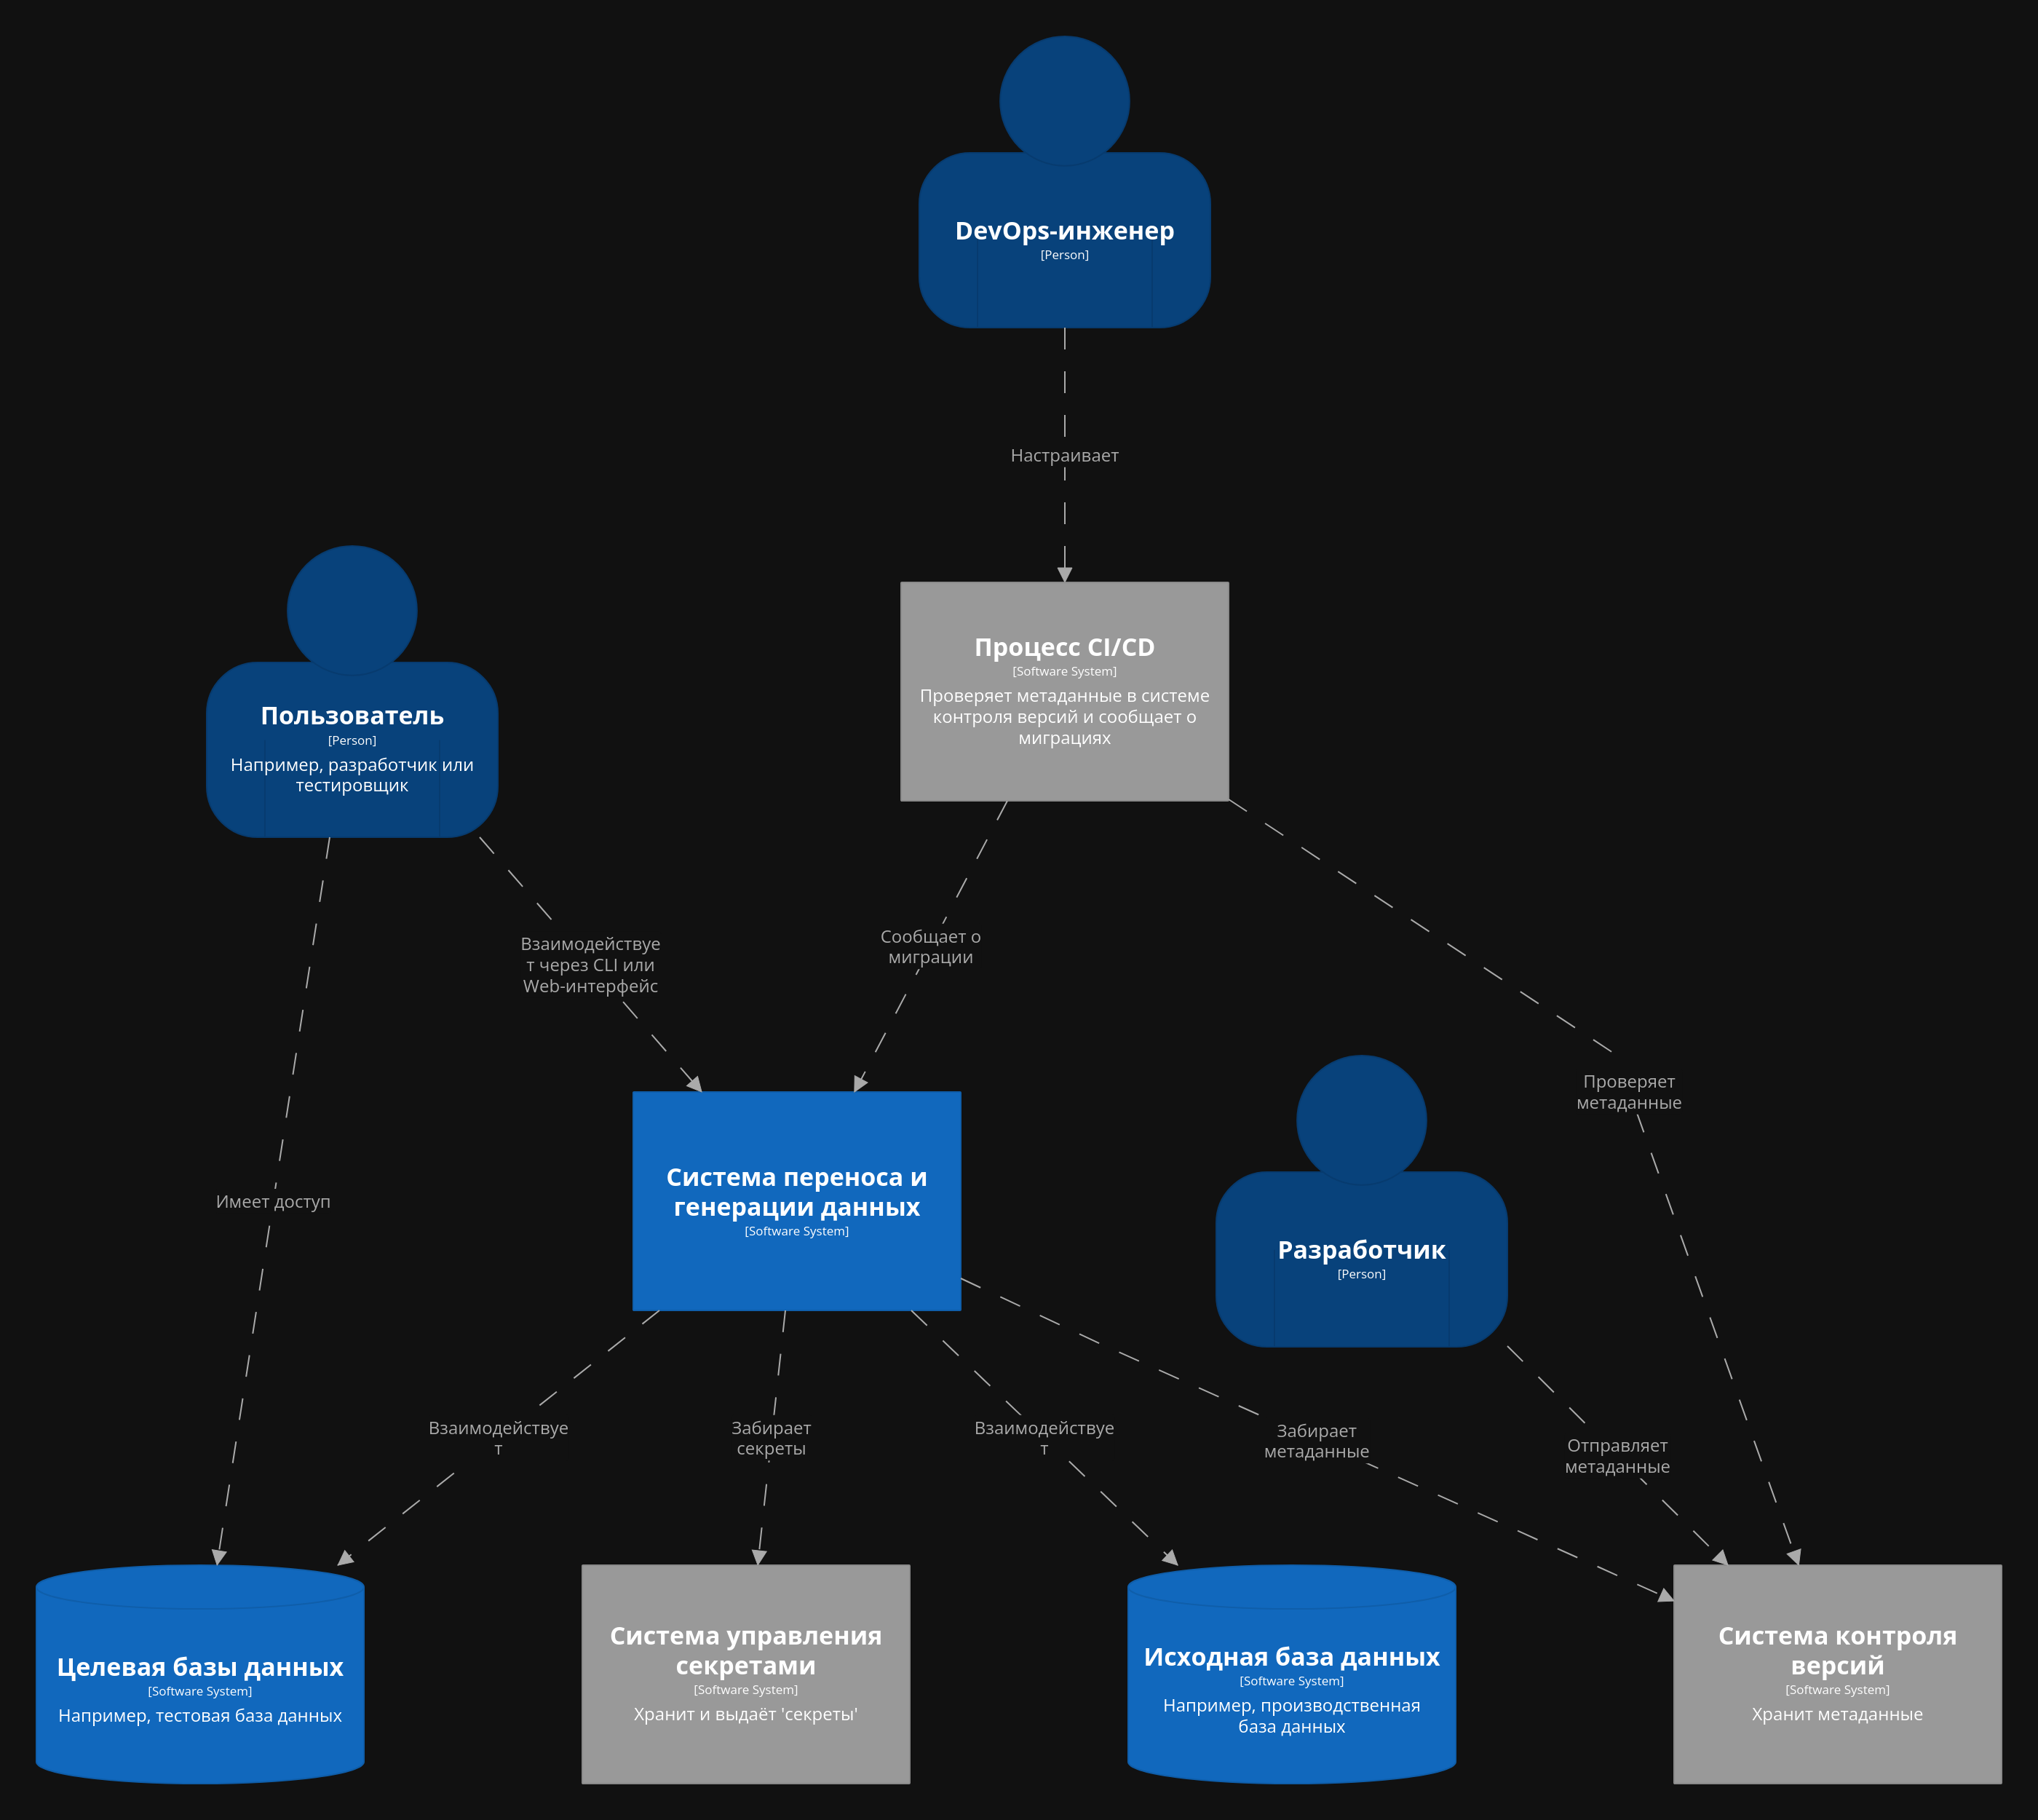
\includegraphics[scale=0.15]{./img/structurizr-SystemLandscape.png}
  \caption{Взаимодействие систем}
  \label{System Context}
\end{figure}

На уровне контекста можно наблюдать взаимодействие различных систем, а также взаимодействие этих систем с пользователями и специалистами.

Внешние системы выделены серым цветом:
\begin{itemize}
\item система контроля версий выступает в качестве хранилища метаданных, представленных разработчиком;
\item система управления секретами предоставляет данные для подключения к базе данных;
\item процесс CI/CD, который настраивает DevOps-инженер, выполняет несколько функций:
  \begin{itemize}
    \item генерация тестовой среды и запуск автоматизированных тестов при получении запроса на слияние в систему контроля версий;
    \item проверка корректности метаданных в момент их фиксации в системе контроля версий;
    \item при выполнении миграций осуществляется уведомление системы переноса и генерации данных о процессах миграции -- это необходимо для предотвращения неопределенного поведения, которое может возникнуть, если система в текущий момент работает с мигрируемой базой данных.
  \end{itemize}
\end{itemize}

Синим цветом выделены собственные системы: исходная и целевая базы данных, с которыми осуществляется взаимодействие пользователей, а также система переноса и генерации данных, которую мы рассмотрим более детально далее.

\subsubsection{Система переноса и генерации данных}

\begin{figure}
  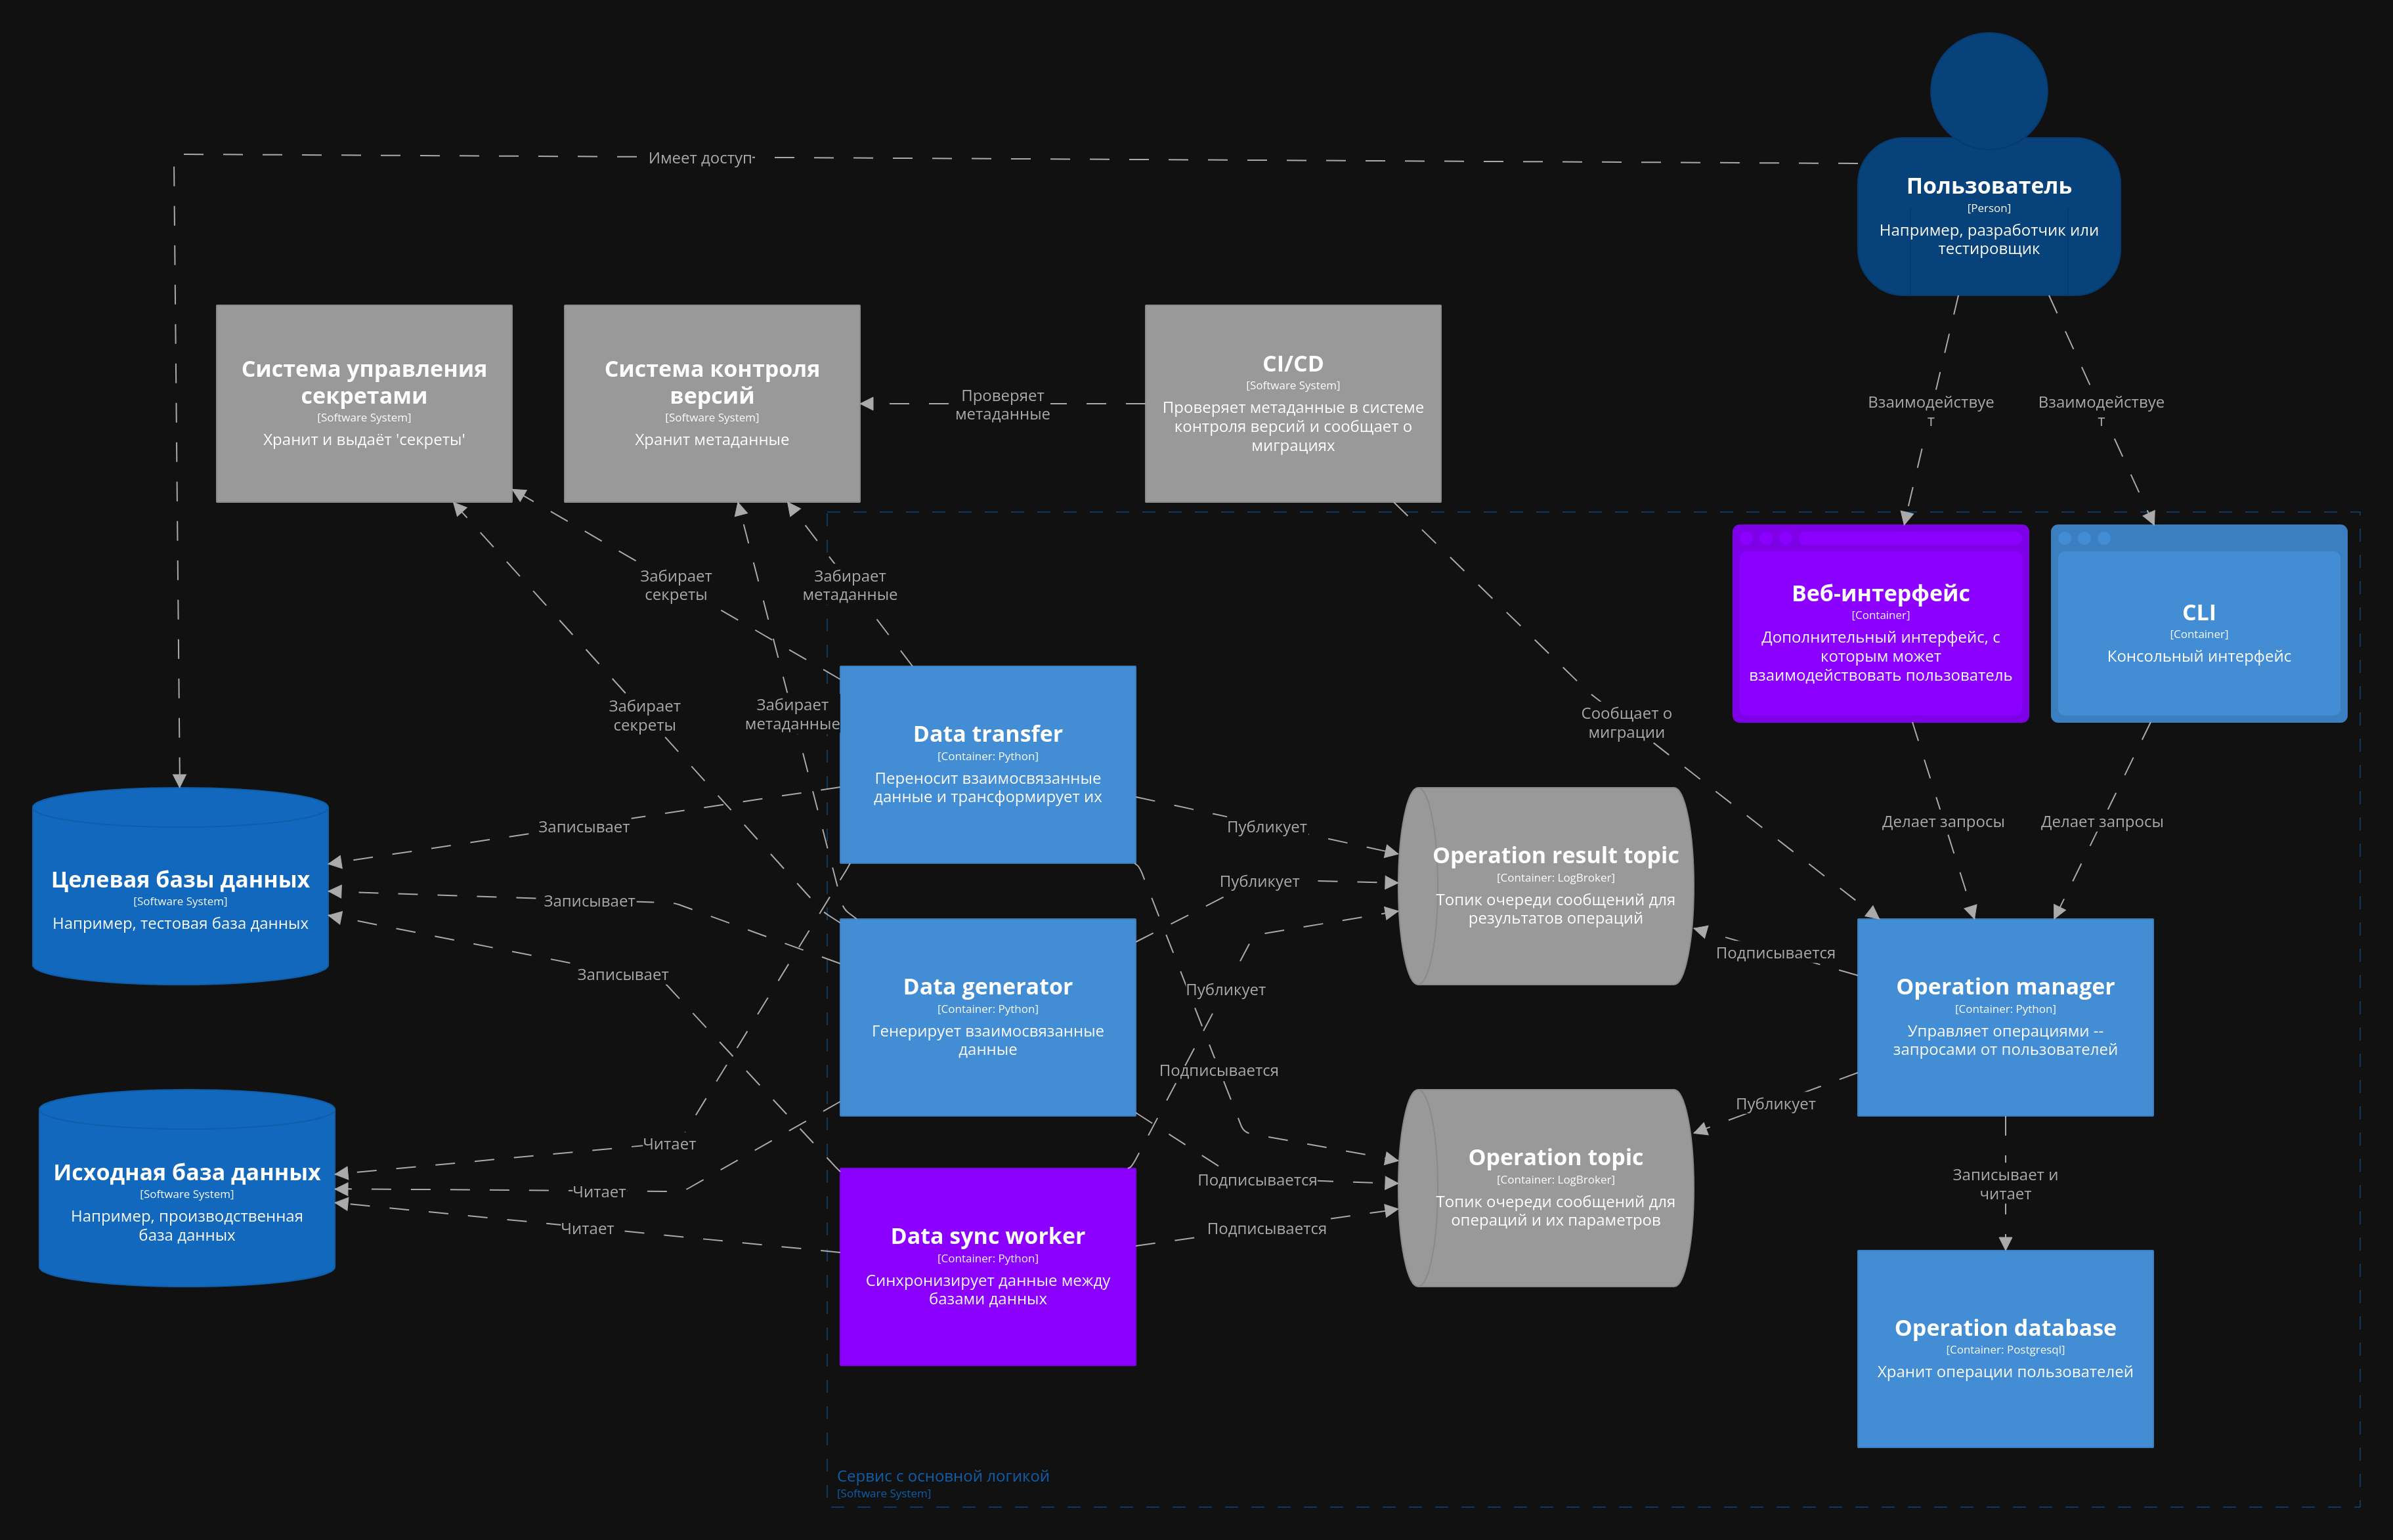
\includegraphics[scale=0.12]{./img/structurizr-Containers.png}
  \caption{Система переноса и генерации данных}
  \label{Containers}
\end{figure}

Рассмотрим систему переноса и генерации данных на уровне контейнеров.

Взаимодействие пользователя с системой осуществляется через командную строку (CLI), хотя может быть реализован и альтернативный интерфейс взаимодействия, например, веб-интерфейс (выделен фиолетовым как контейнер, который может быть добавлен в перспективе).

Пользователь посылает запросы в контейнер Operation Manager. Возможны два типа запросов: запуск операции по переносу или генерации данных, а также проверка статуса выполняемой операции. В случае получения запроса на запуск операции, информация об операции сохраняется в базе данных, а уникальный идентификатор операции возвращается пользователю, что позволяет ему отслеживать статус выполнения.

Далее Operation Manager отправляет запросы на выполнение операции в очередь сообщений Logbroker~\cite{logbroker}. Контейнер, обрабатывающий такой запрос, определяется типом операции: если речь идет о переносе данных, операция обрабатывается контейнером Data Transfer; если о генерации данных — контейнером Data Generator.

На схеме также представлен контейнер Data Sync Worker, являющийся гипотетическим контейнером, предназначенным для обработки операций по синхронизации данных в базах данных.

Контейнеры Data Transfer и Data Generator осуществляют перенос и генерацию данных, взаимодействуя с базами данных, системой контроля версий и системой управления секретами. В процессе выполнения операции, а также после её выполнения, информация о статусе возвращается в очередь сообщений, из которой Operation Manager извлекает данные и обновляет статус операции в базе данных.

Более детальное описание структуры компонентов Data Transfer и Data Generator будет представлено в последующих разделах.

Рассмотрим диаграмму последовательности взаимодействия пользователя с системой на примере генерации данных.

\begin{figure}
  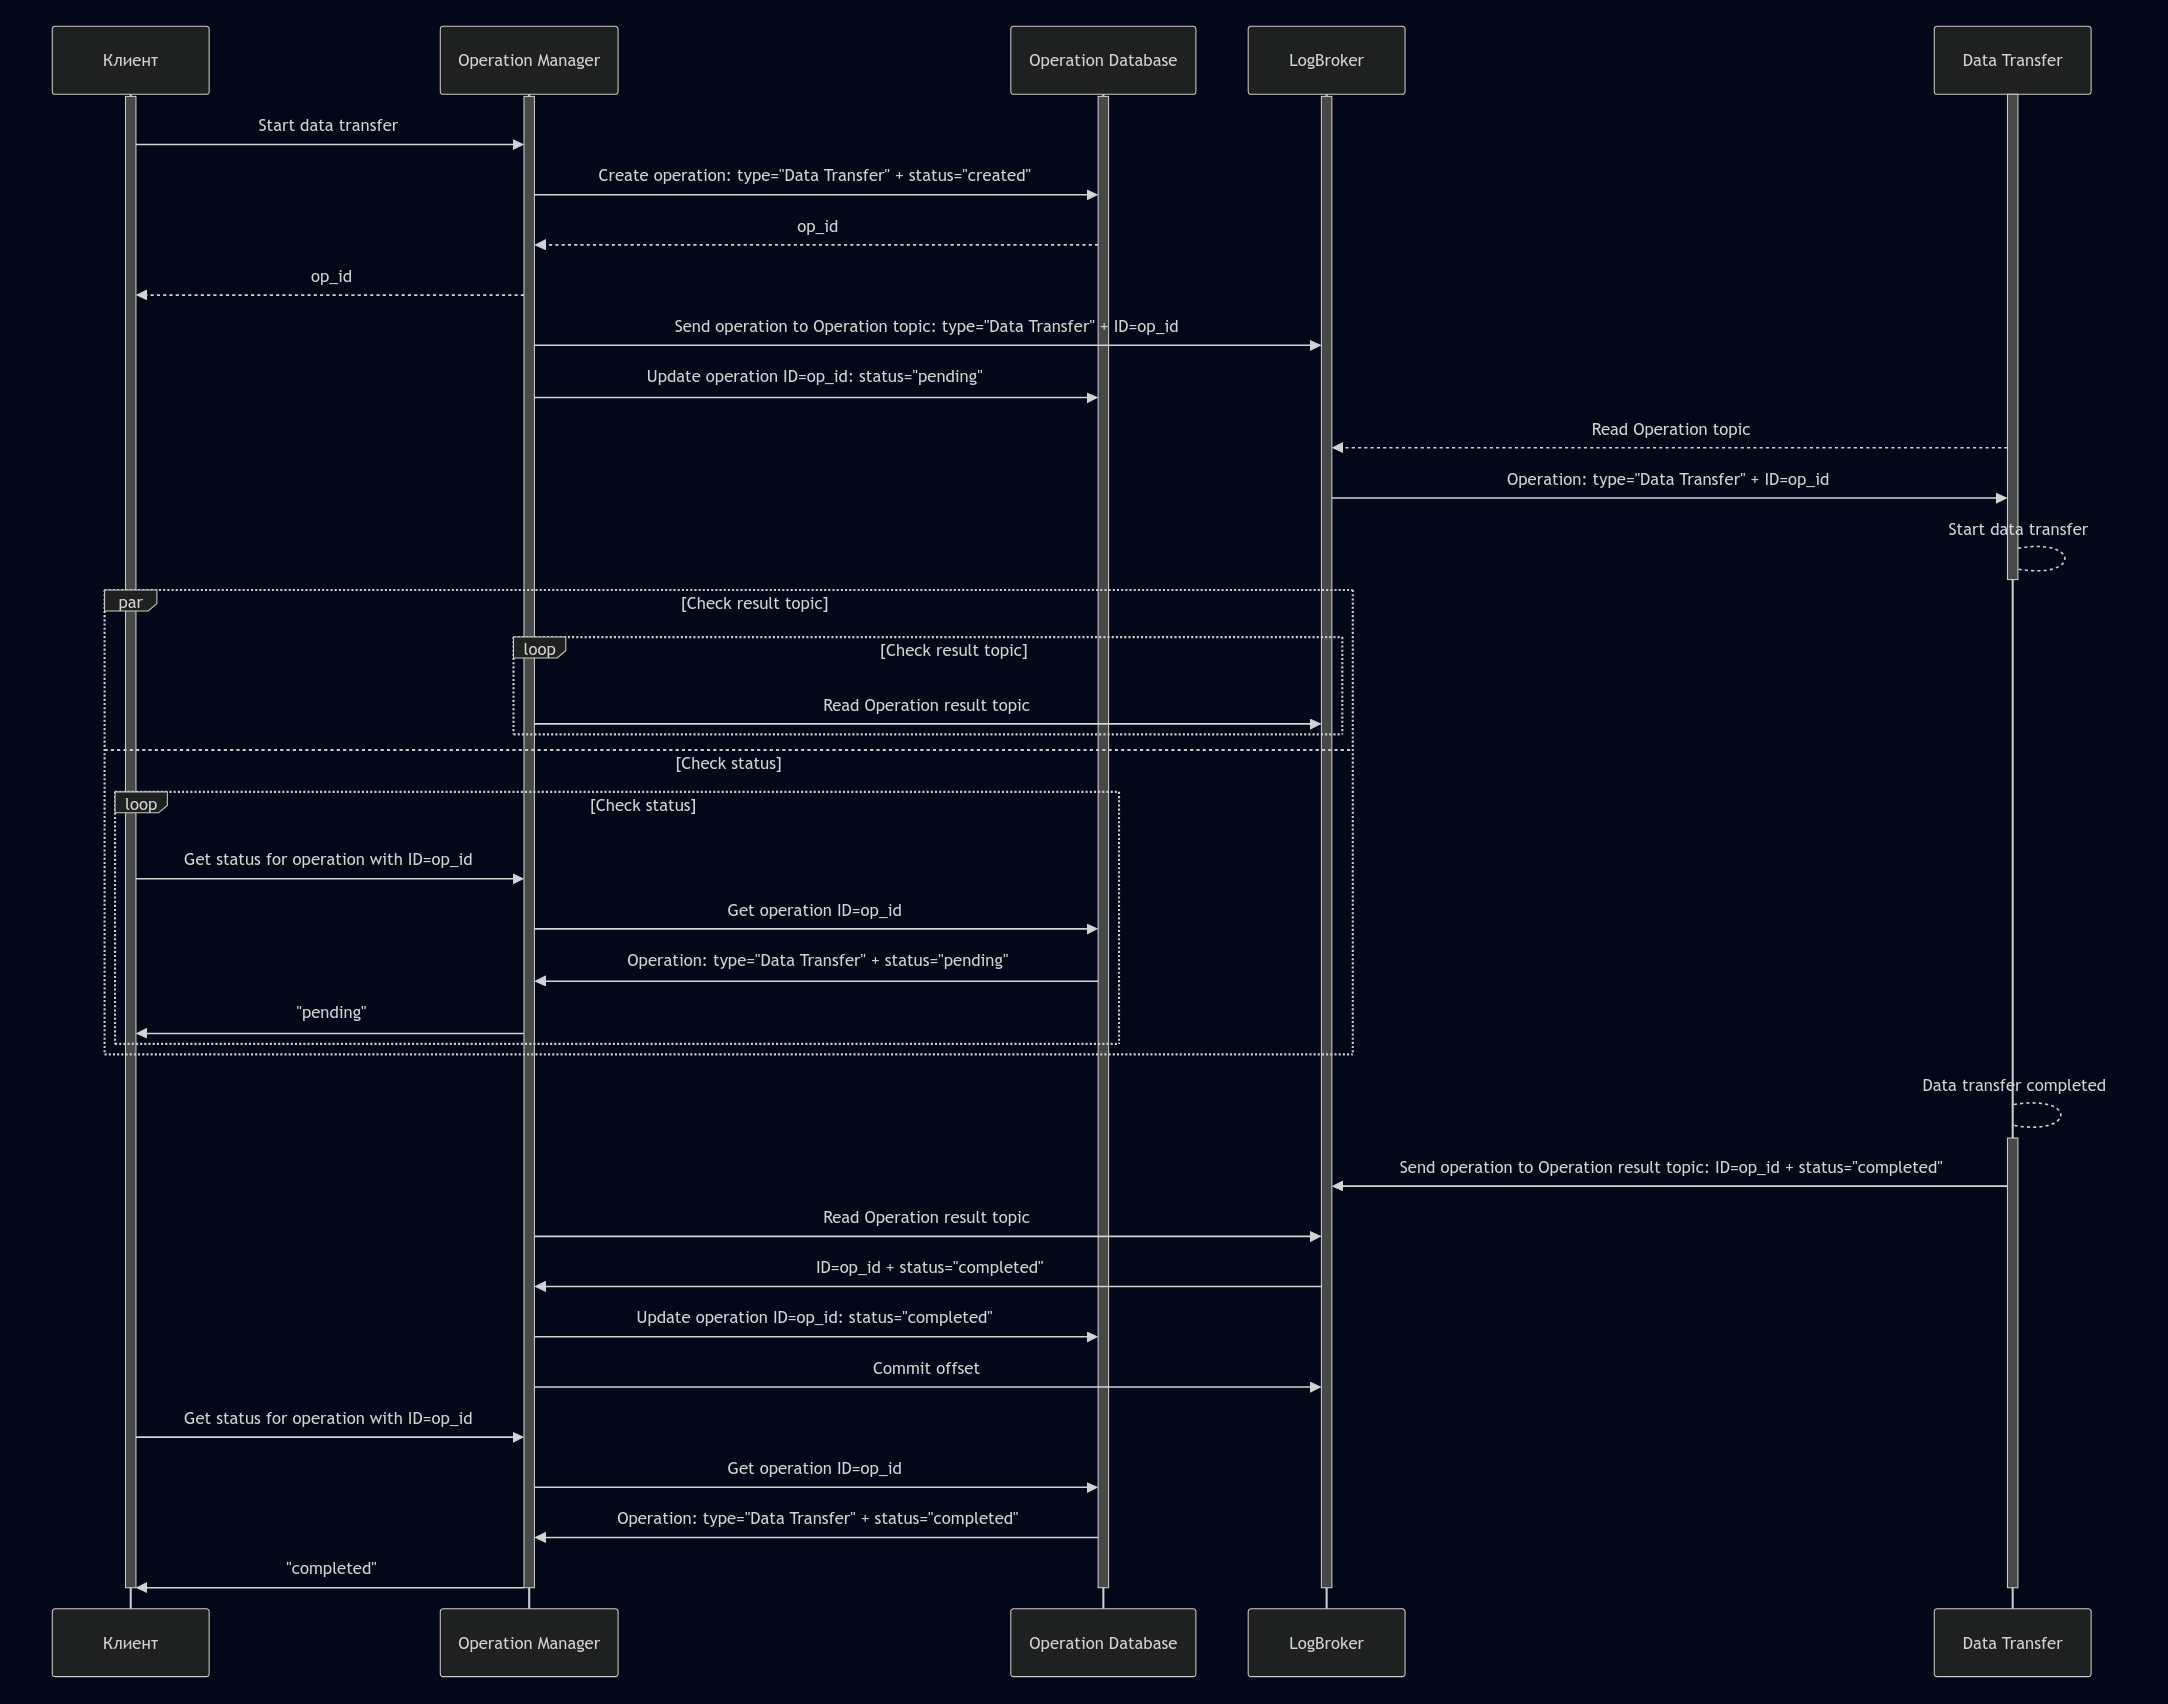
\includegraphics[scale=0.2]{./img/mermaid-sequence-User-MainSystem.png}
  \caption{Диаграмма последовательности взаимодействия пользователя с системой на примере генерации данных}
  \label{Sequence User-MainSystem}
\end{figure}

На диаграмме можно заметить, как клиент и система общаются асинхронно.

\subsubsection{Компоненты переноса данных}

\begin{figure}
  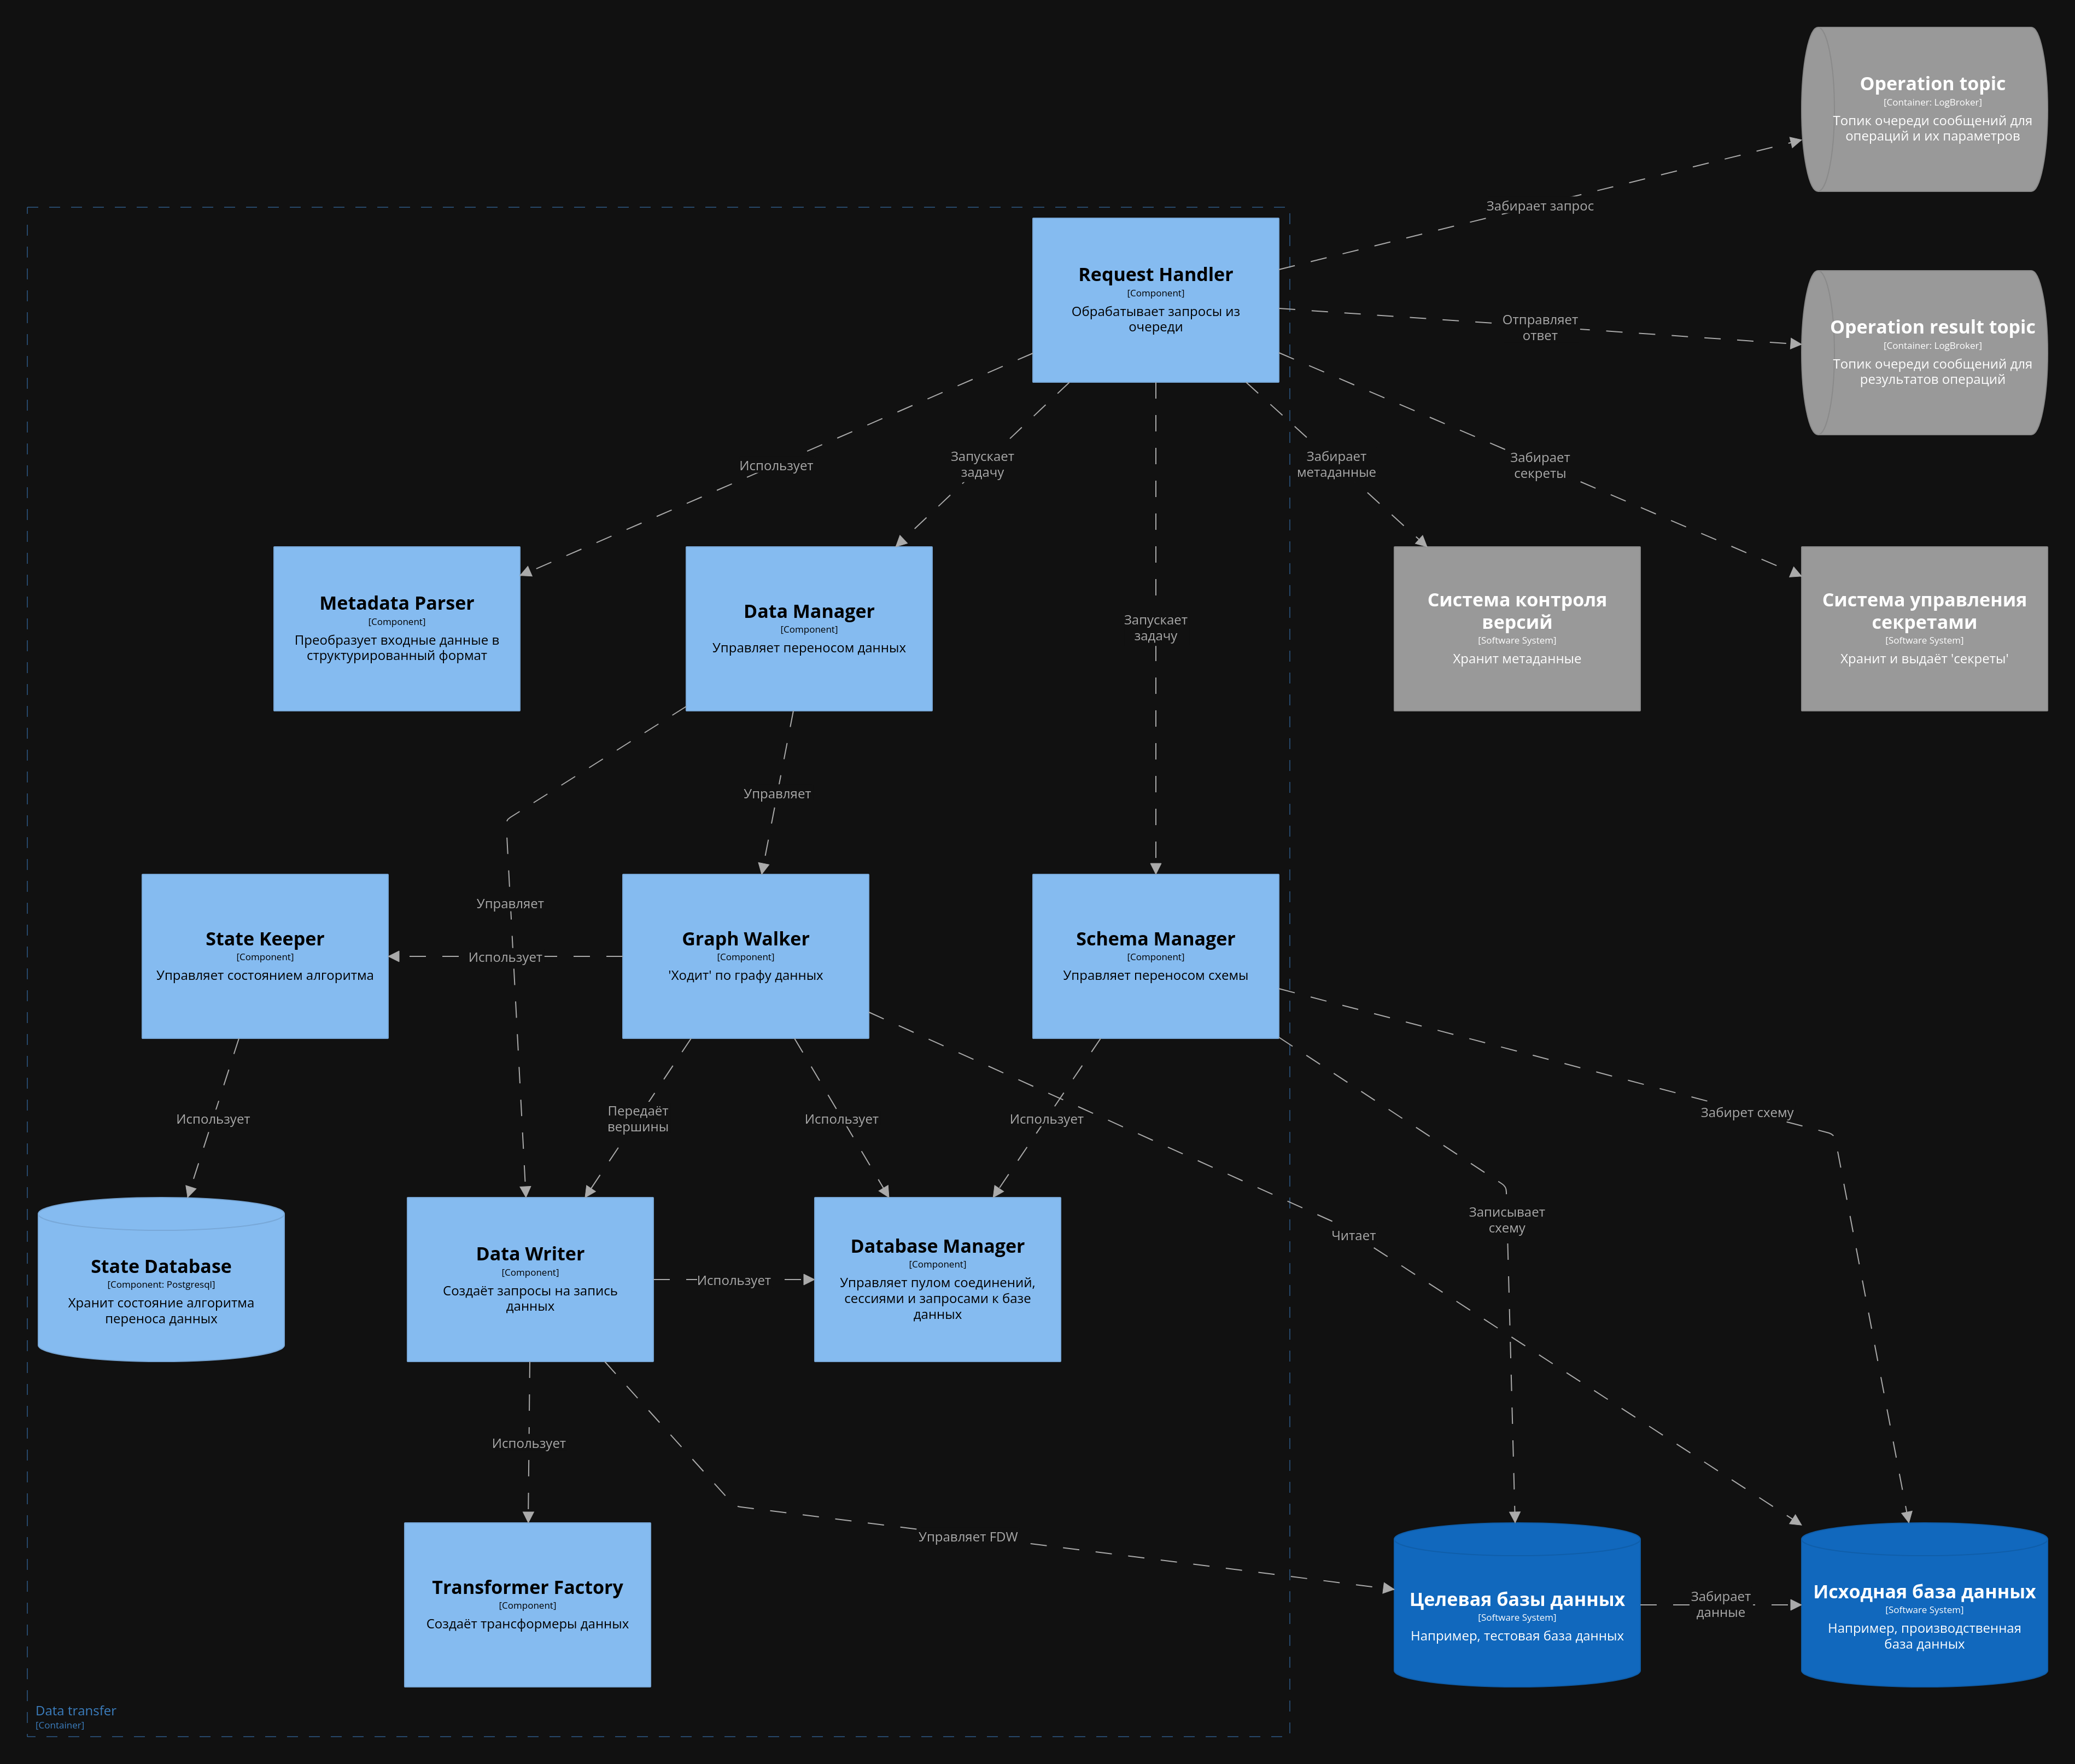
\includegraphics[scale=0.12]{./img/structurizr-DataTransferComponents.png}
  \caption{Компоненты Data Transfer}
  \label{Data Transfer Components}
\end{figure}

Рассмотрим процесс обработки запросов на перенос задач. Компонент Request Handler принимает такие запросы. Они должны включать следующие элементы:

\begin{itemize}
  \item идентификатор метаданных;
  \item идентификатор исходной базы данных;
  \item идентификатор целевой базы данных.
\end{itemize}

Идентификатор метаданных может принимать форму одной из двух сущностей: уникального идентификатора, связанного с метаданными в Системе контроля версий, или самих метаданных. В случае предоставления уникального идентификатора, Request Handler обращается к Системе контроля версий для извлечения соответствующих метаданных.

Идентификатор базы данных может быть представлен либо в форме уникального идентификатора кластера базы данных, либо в виде параметров подключения к базе данных. При предоставлении уникального идентификатора кластера базы данных, Request Handler обращается к Системе управления секретами для получения необходимых параметров подключения, включая пароль.

Полученные метаданные направляются в компонент Metadata Parser для их валидации и преобразования во внутренний формат представления. Далее инициируется Data Manager, который получает информацию о подключениях к базам данных, а также внутреннее представление метаданных, и запускает компоненты Graph Walker и Data Writer.

Компонент Graph Walker выполняет алгоритм обхода данных исходной базы, который будет рассмотрен позже, следуя инструкциям, заданным в метаданных. Он использует State Keeper для сохранения состояния алгоритма и Database Manager для выполнения операций с базой данных. В процессе работы, Graph Walker извлекает метаинформацию о посещенных вершинах и асинхронно передает её компоненту Data Writer.

Компонент Data Writer управляет преобразованием данных и их записью в целевую базу данных. Он принимает на вход метаинформацию о данных, включая их идентификаторы, и с помощью Database Manager создаёт объект Foreign Data Writer~\cite{fdw} в целевой СУБД, обеспечивая прямое подключение к исходной СУБД. Data Writer формирует запросы, включающие идентификаторы данных, направляя их в целевую СУБД для извлечения конкретных данных из исходной базы. Запросы дополняются трансформерами, сформированными на основе метаданных через компонент Transformer Factory. Трансформер представляет собой набор правил преобразования данных, например, для анонимизации данных.

Рассмотрим взаимодействие основных компонент на диаграмме последовательности.

\begin{figure}
  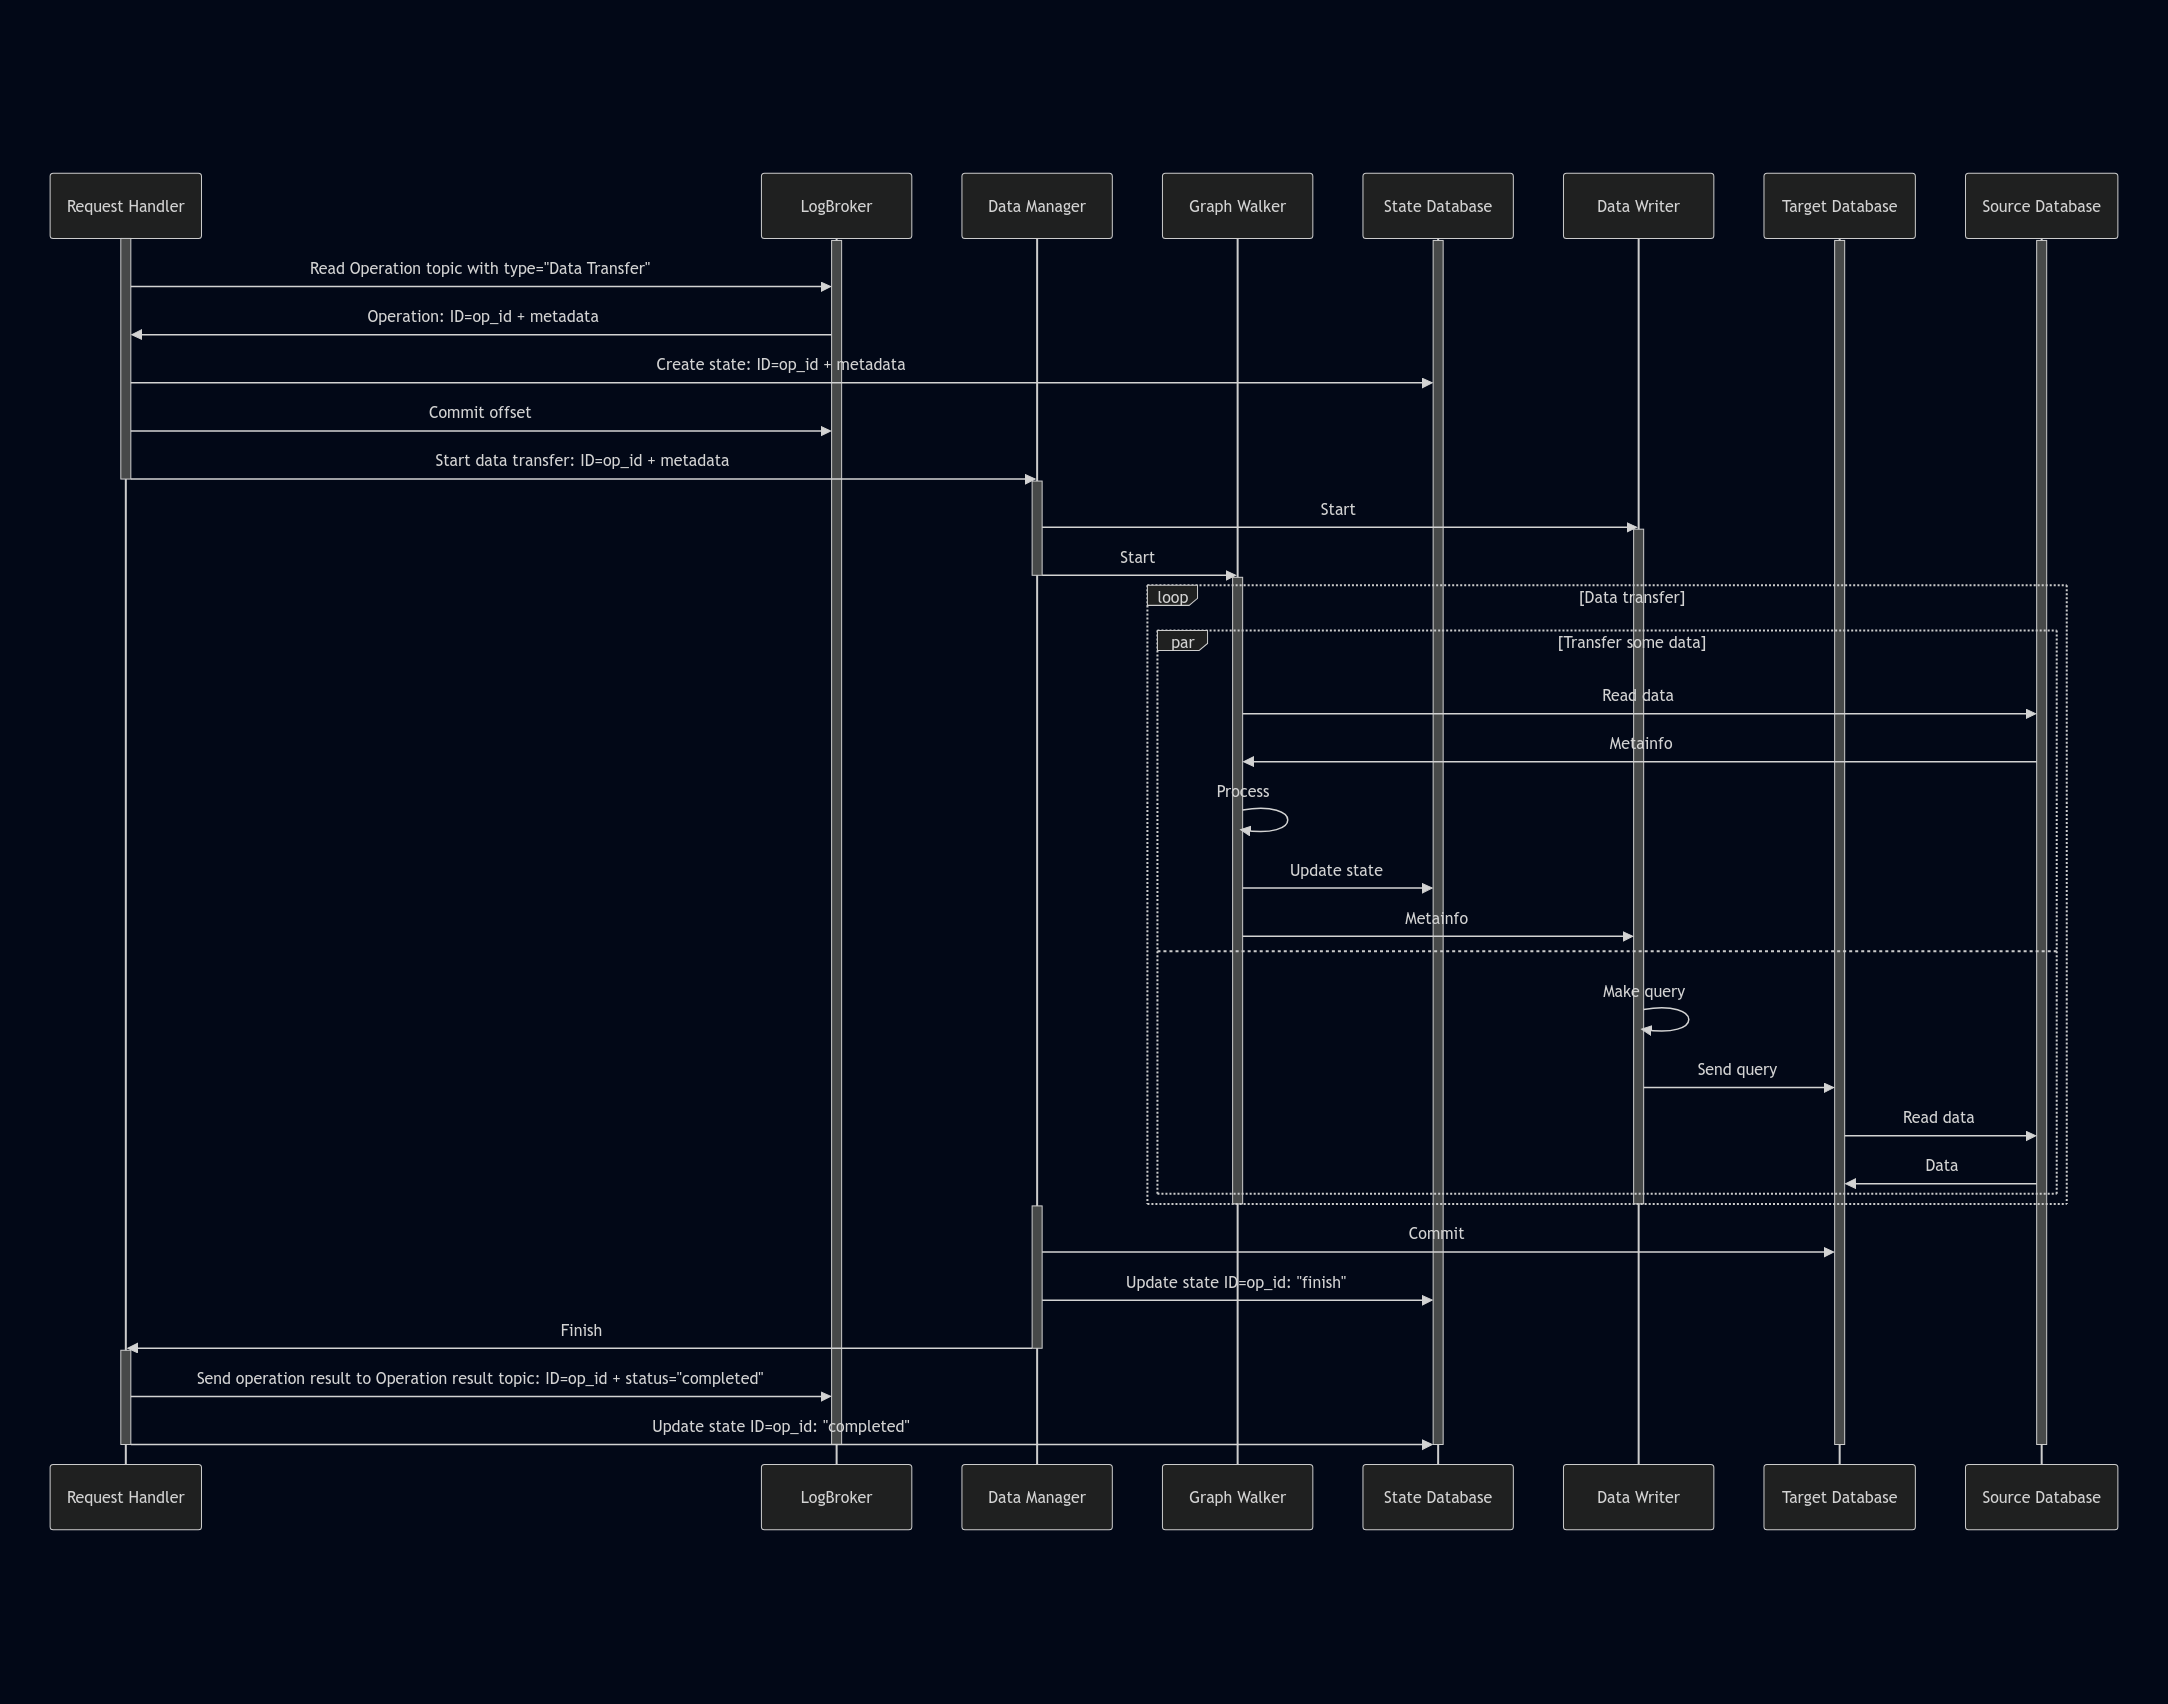
\includegraphics[scale=0.2]{./img/mermaid-sequence-DataTransfer.png}
  \caption{Диаграмма последовательности взаимодействия пользователя с системой на примере генерации данных}
  \label{Sequence DataTransferComponents}
\end{figure}

Данный подход предусматривает непосредственный перенос данных из исходной базы в целевую, с возможными изменениями в соответствии с правилами, определёнными в метаданных, что способствует повышению производительности системы.

Также на рисунке~\ref{Data Transfer Components} представлен компонент Schema Manager, который предоставляет функциональность по управлению схемами баз данных. В частности, данный компонент позволяет осуществлять перенос схемы между различными базами данных, а также выполнять удаление схемы.

\subsubsection{Компоненты генерации данных}

\begin{figure}
  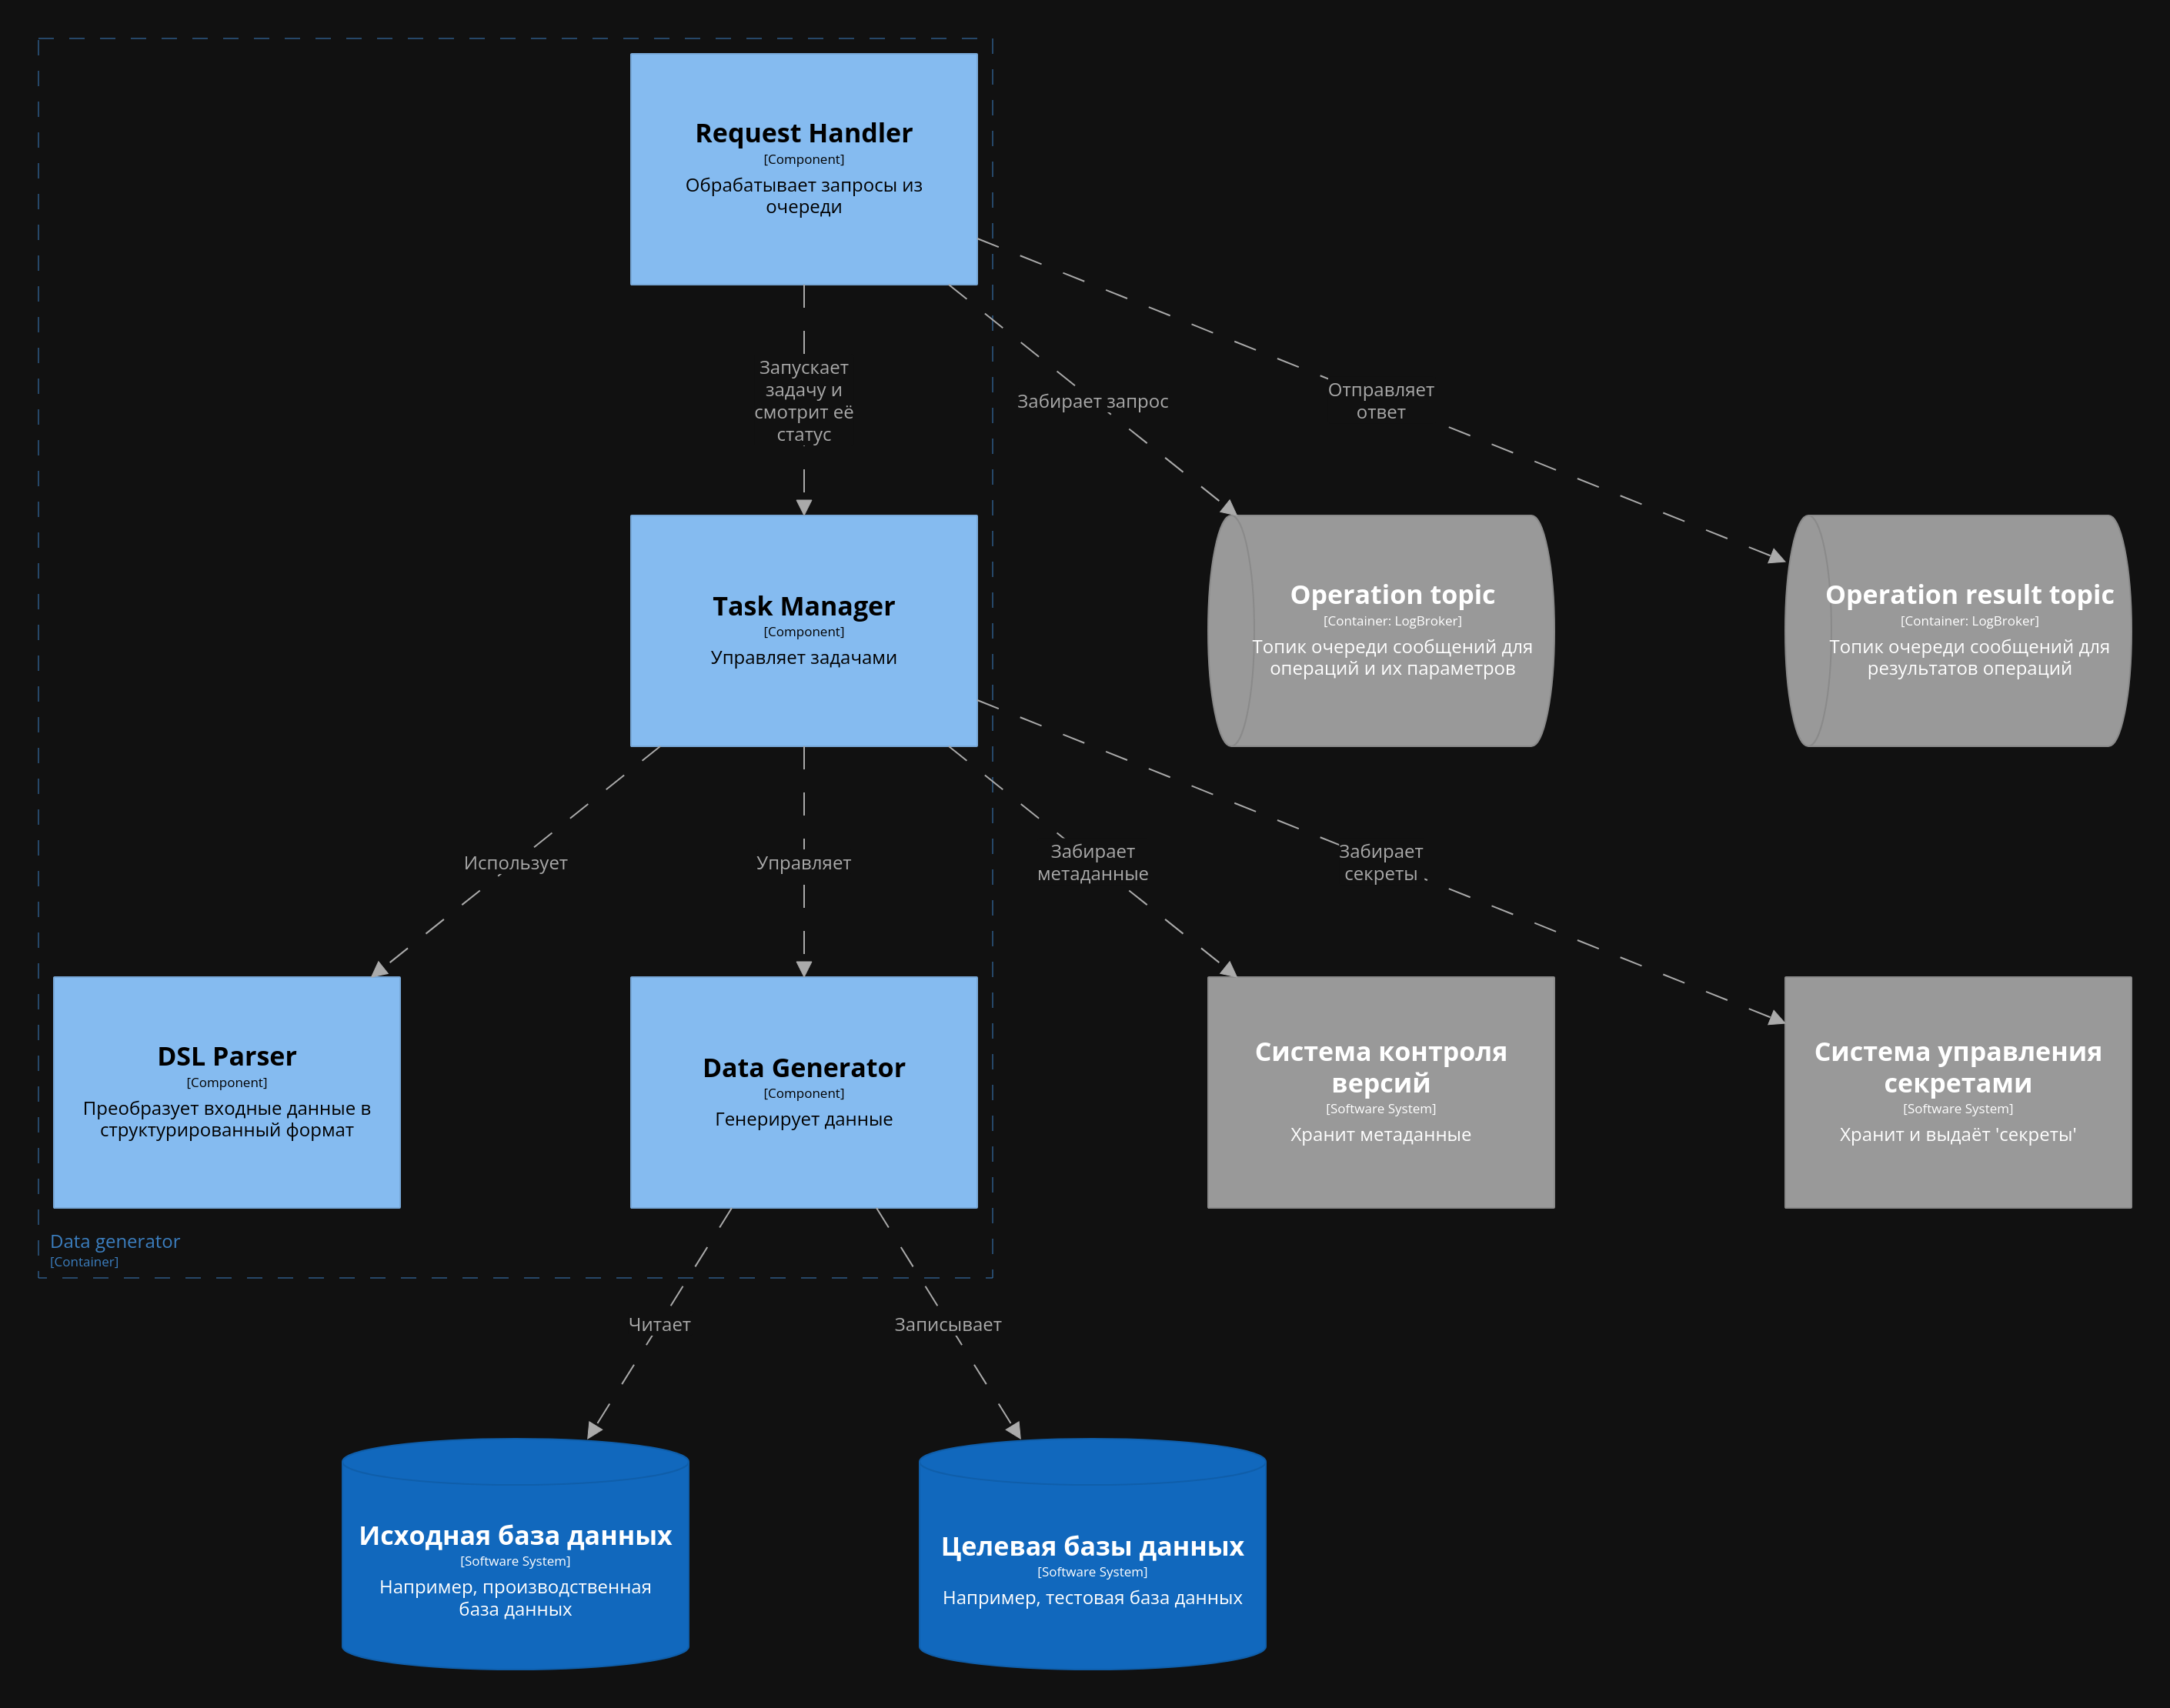
\includegraphics[scale=0.15]{./img/structurizr-DataGeneratorComponents.png}
  \caption{Компоненты Data Generator}
  \label{Data Generator Components}
\end{figure}

TBD: расписать взаимодействие компонент Data generator

\subsubsection{Персистентность состояния и восстановление после сбоя}

Процессы переноса данных могут быть времязатратными, независимо от объёма данных. В случае неожиданной остановки сервиса переноса и генерации данных, вызванной сбоем, утрата прогресса по переносу данных становится крайне нежелательным исходом.

Рассмотрим, как выполняется персистентность состояния системы, то есть её способность сохранять и восстанавливать своё состояние после остановки.

Весь процесс выполнения операции от её инициации до её завершения можно разделить на два этапа:
\begin{itemize}
  \item отправка и чтение из очереди сообщений;
  \item непосредственный процесс переноса данных.
\end{itemize}

Сбои могут возникать на любом из этих этапов. Для этапа отправки и чтения сообщений из очереди предусмотрена семантика доставки exactly-once~\cite{delivery-guarantees}, которая поддерживается использованием архитектурных паттернов Inbox Pattern и Outbox Pattern~\cite{outbox-and-inbox}. Эти паттерны, часть реализации которых можно наблюдать на диаграммах последовательностей~\ref{Sequence User-MainSystem} и~\ref{Sequence DataTransferComponents}, обеспечивают гарантированную доставку сообщений и идемпотентную обработку входящих данных.

При сбое на этапе переноса данных механизмы восстановления включают проверку состояния незавершённых операций в базе данных состояния (State Database). В ней хранится прогресс каждой операции переноса данных и включает уникальные идентификаторы операции, состояние алгоритма и метаданные. При восстановлении система переноса данных проверяет наличие незавершённых операций и продолжает их с того места, где процесс был остановлен. Запись в целевую базу данных успешно завершается только при успешном выполнении алгоритма, что требует повторной записи данных в случае восстановления после сбоя, основываясь на метаинформации из сохранённого состояния.

Таким образом, архитектура системы включает механизмы обеспечения персистентности состояния и восстановления после сбоев.

\subsubsection{Безопасность}

TBD: расписать, как выполняется свойство безопасности системы

\subsection{Алгоритм обхода данных}

Всю основную функциональность переноса данных можно разделить на две части: запись данных в целевую базу данных, которую мы рассматривали ранее, и обход исходных данных, алгоритм которого мы рассмотрим подробнее в этом разделе.

\subsubsection{Метаграфы}
На сегодняшний день в научном сообществе не существует общепринятого и устойчивого определения метаграфа. Работа \cite{metagraphs_1} была первым источником, в котором появился термин "метаграф". Эта концепция всё ещё находится в стадии развития и интерпретируется различными исследователями по-разному в зависимости от их специфических задач и целей \cite{metagraphs_2}~\cite{metagraphs_3}~\cite{metagraphs_4}~\cite{metagraphs_5}. В общем смысле, метаграф можно рассматривать как структуру, которая обобщает и расширяет идеи классических графов, чтобы решить более сложные задачи анализа данных и моделирования.

В данной дипломной работе предлагается собственное определение метаграфа, адаптированное под требования и задачи рассматриваемого алгоритма.

$MG = <V, MV, E, ME>$ -- метаграф, где $V$ -- множество вершин, $MV$ -- множество метавершин, $E$ -- множество рёбер, $ME$ -- множество метарёбер.

$v_i = \{atr_k\}, v_i \in V$, где $v_i$ -- вершина, $atr_k$ -- атрибут.

$mv_i = <\{v_j\}, \{atr_k\}>, mv_i \in MV, v_j \in V$, где $mv_i$ -- метавершина, $v_j$ -- вершина, $atr_k$ -- атрибут.

$e_i = <v_s, v_e>, e_i \in E, v_s, v_e \in V$, где $e_i$ -- ребро, $v_s$ -- исходная вершина, $v_e$ -- конечная вершина.
$me_i = <mv_s, mv_e, \{atr_k\}>, me_i \in ME, mv_s, mv_e \in MV$, где $me_i$ -- метаребро, $mv_s$ -- исходная метавершина, $mv_e$ -- конечная метавершина, $atr_k$ -- атрибут.

Также введём ограничение на множество метавершин: $\forall mv_i, mv_j \in V, i \neq j => \{v_x\}_i \cap \{v_y\}_j = \emptyset$, т.е. каждая вершина не может содержаться в нескольких метавершинах.

\subsubsection{Представление базы данных в виде метаграфа}

Реляционные базы данных традиционно состоят из множества связанных таблиц, каждая из которых содержит структурированные данные. В метаграфе эти элементы могут быть представлены следующим образом.

\begin{itemize}
  \item Метавершины. В контексте метаграфа метавершинам соответствуют конкретные таблицы реляционной базы данных. Набор атрибутов метавершины содержат информацию о структуре таблицы, включая её название, идентификатор и набор столбцов.

  \item Вершины. Вершины, представляющие собой элементы более низкого уровня в сравнении с метавершинами, соответствуют записям в таблицах. Каждый набор атрибутов вершины напрямую соответствует набору значений в конкретной записи таблицы.

  \item Метарёбра. Метарёбра описывают связи между различными таблицами в базе данных. Эти связи формируются посредством внешних ключей~\cite{foreign-key}, которые указывают на зависимость одной таблицы от другой. Атрибуты метарёбер содержат информацию о полях, которые связаны между таблицами, что создаёт основу для передачи данных и взаимозависимости структур.

  \item Рёбра. Рёбра представляют связи между конкретными записями в таблицах и формируются на основании соответствующих метарёбер. Эти рёбра конкретизируют связь на уровне данных, отражая указанные в метарёбрах отношения через конкретные внутренние связи записей, например, через одинаковые или согласованные идентификаторы.
\end{itemize}

Для иллюстрации представления базы данных в виде метаграфа рассмотрим небольшой пример, содержащий пять таблиц по несколько записей в каждой.

\begin{figure}
  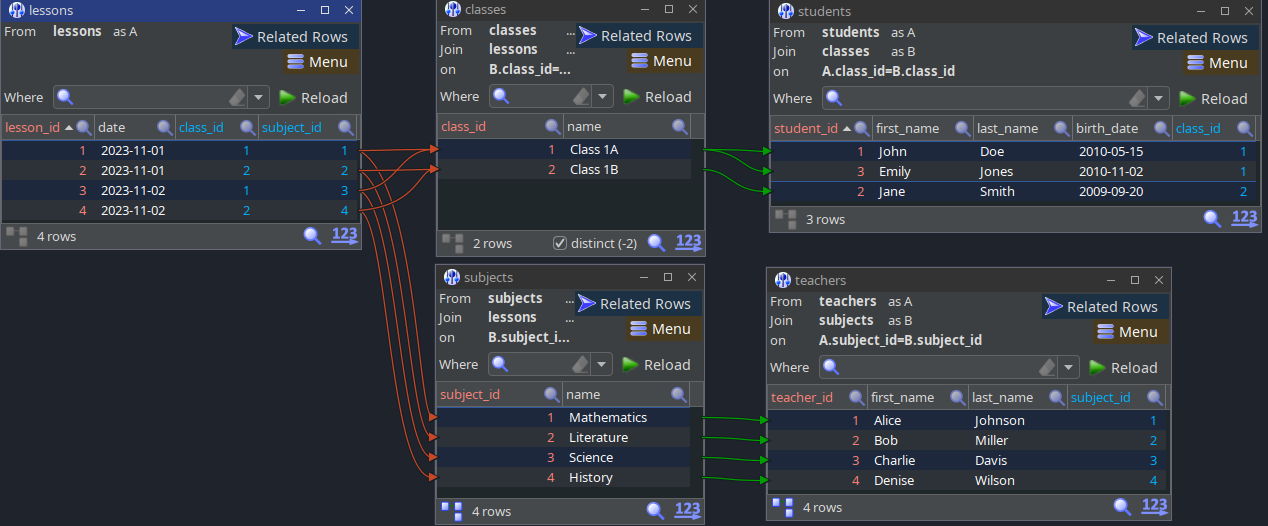
\includegraphics[scale=0.5]{./img/jailer-example-db-overview.png}
  \caption{Пример реляционной базы данных}
  \label{db-example}
\end{figure}

На рисунке \ref{db-example} представлена схема взаимосвязей между конкретными записями в базе данных. Красные стрелки указывают на то, что записи, из которых исходят стрелки, имеют ссылки на другие записи. Это свидетельствует о наличии во внешней таблице внешнего ключа, ссылающегося на другую таблицу. В свою очередь, зелёные стрелки обозначают противоположную ситуацию: данные, на которые они указывают, являются объектом ссылок со стороны других записей.

Рассмотрим метаграф, соответствующий заданной базе данных.

\begin{figure}
  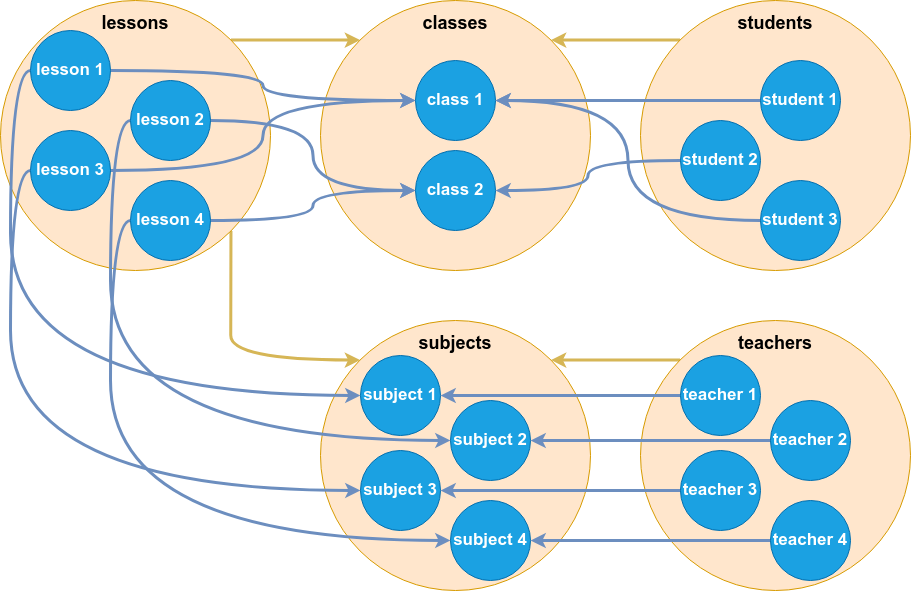
\includegraphics[scale=0.5]{./img/drawio-metagraph-overview.png}
  \caption{Пример метаграфа}
  \label{metagraph-example}
\end{figure}

На рисунке \ref{metagraph-example} представлено графическое изображение метаграфа. Оранжевым цветом обозначены метавершины и метарёбра, которые соответствуют таблицам и связям между этими таблицами. В свою очередь, синим цветом представлены вершины и рёбра, отражающие записи и связи между ними.

\subsubsection{Описание базового алгоритма}
Необходимо уметь проходить по взаимосвязанным данным. Поскольку теперь можно представить базу данных в виде метаграфа, алгоритм обхода данных фактически будет являться алгоритмом обхода графа.

Такой алгоритм должен принимать на вход множество начальных вершин, которые соответствуют конкретным данным, а также метаграф, представляющий базу данных. На выходе алгоритм должен предоставлять множество всех вершин, связанных с начальными, включая сами начальные вершины.

В качестве основного алгоритма для решения поставленной задачи предлагается использовать метод поиска в ширину. Данный подход позволяет эффективно обрабатывать структуры данных, представленные в виде графов. Следует отметить, что псевдокод алгоритма разработан на основе соглашений и обозначений, представленных в \cite{kormen-algorithms}.

\begin{figure}
  \begin{lstlisting}
Base_Search_For_Relational_Data(DB, SV)
  Queue := {}
  Visited := {}
  for each v in SV
    do ENQUEUE(Q, v)
  while Queue != {}
    do cur_v := DEQUEUE(Queue)
        ADD(Visited, cur_v)
        for each u in ADJACENT(DB, cur_v)
          do if u NOTIN Visited:
            then ENQUEUE(Queue, u)
  return Visited
  \end{lstlisting}
  \caption{Базовый алгоритм поиска взаимосвязанных данных}
\end{figure}

Говоря о представленном выше описании, отметим следующие моменты:
\begin{itemize}
  \item алгоритм принимает на вход два параметра: метаграф \textit{DB}, который представляет собой базу данных, и множество начальных вершин \textit{SV}, с которых начинается поиск;
  \item операция \textit{ENQUEUE(Q, x)}} предусматривает добавление элемента \textit{x} в конец очереди \textit{Q};
  \item операция \textit{DEQUEUE(Q)} удаляет элемент из начала очереди \textit{Q};
  \item операция \textit{ADD(S, x)} добавляет элемент \textit{x} в множество \textit{S};
  \item функция \textit{ADJACENT(MG, x)} возвращает множество вершин, которые являются смежными с вершиной \textit{x} в метаграфе \textit{MG}, идентифицируя потенциалы для дальнейшего обхода.
\end{itemize}



\subsubsection{Устройство Postgresql}
TBD: здесь хочу описать некоторые моменты из устройства Postgresql: ctid, tableoid -- они применяются в имплементации алгоритма.

\subsubsection{Имплементация}
TBD: здесь хочу наложить алгоритм на Postgresql и написать имплементацию алгоритма на Python (которая уже готова, но её просто так нельзя выкладывать :D).

\subsection{Генерация данных}
TBD: генерация данных далеко не основная функциональность системы, поэтому времени ей будет уделено немного

\subsection{Разработка языка}
TBD: есть синтаксис языка, но нужно реализовать парсер. Структура этого раздела пока под вопросом

\subsubsection{Синтаксис и грамматика языка}

\subsubsection{Корректность языка}

\subsubsection{Язык задания графа}

\subsubsection{Язык переноса данных}

\subsubsection{Язык генерации данных}
